\chapter{When It Won't Fit: Working with Secondary Stores}

When you've tried every trick in the book, and your data still does not fit
within the constraints of available memory or address space, your remaining
option is to shuttle it in and out of the heap. While a subset of your data is
stored in the heap, the entirety of the data needs to be persisted on some kind
of \emph{secondary storage} device. Commonly, data is persisted as files on a
local filesystem or a distributed filesystems such as Hadoop's HDFS, in
flat-file data stores such as sqlite or Berkeley db, as key-value pairs in
distributed in-memory caches such as memcached, as tuples in a directory server,
or tables in a relational database. You have lots of options!

Most often, the choice you make of how to store the data dictates how you get
the data to and from the secondary store. The provider of the storage mechanism
usually provides a Java library that implements a data access API. For example,
every relational database comes with code that implements the Java DataBase
Connectivity (JDBC) API. This API takes care of the task of turning database
query results (a list of rows) into Java objects, and vice versa. These
processes are termed \emph{deserialization} and
\emph{serialization}\index{Serialization}. These terms are sometimes
synonymously referred to as the steps of \emph{marshalling} data.\footnote{Some
sticklers distinguish marshalling to be serialization and deserialization along
with a protocol for ensuring compatibility between code releases. In this
lexicon, a marshalled object is a record not only of the data, but also of the
version, or even the schema itself, of serialized form.}

On top of the basic data access layers, there exist a number of libraries that
hide the low-level details that are particular to any one secondary store. Most
JDBC libraries will marshall data to and from Java objects, but these objects
are not the objects you care about. THey are instead quite literal Java
manifestations of relational database concepts: connections, prepared
statements, and result sets. Hibernate, for example, raises the level of
interfacing with relational databases so that you needn't be concerned with
these lower level details.



\section{Serialization: Copying Data in and Out}
\index{Serialization}

When interacting with secondary stores, there are three possible stages of the
data between the in-transit form and your initial java objects: the serialized
form, the in-memory intermediate form, and the initial form of your Java data
modles. There of course may be even more forms of java objects, as the data
flows through the Java code, but these are the three forms of data that are
involved with communicating with secondary stores.

\begin{figure}
\centering
  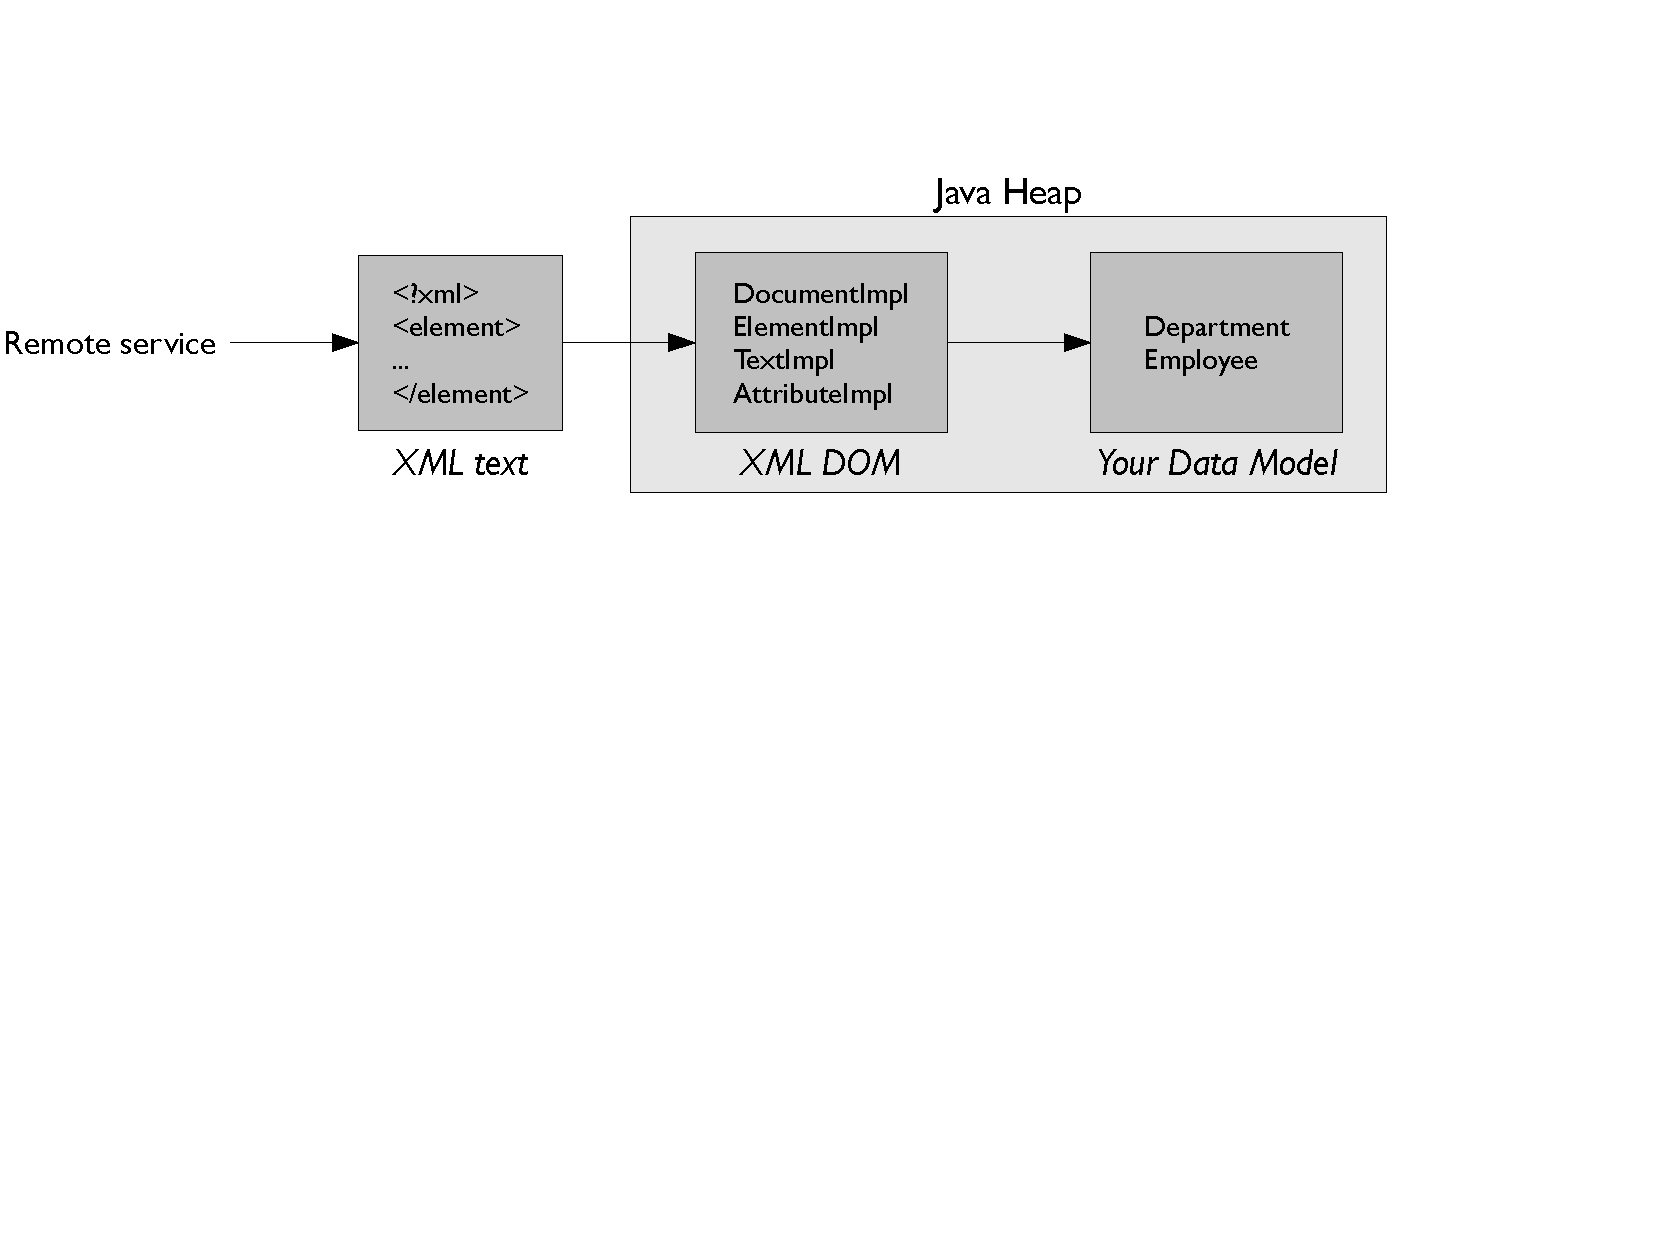
\includegraphics[width=0.95\textwidth]{part3/Figures/secondary/serializationforms}
  \caption{An example of data that takes on three forms as it flows from a
  secondary data source (in this case, a remote service) eventually into your
  Java data model.}
\end{figure}

\begin{itemize}

\item \textbf{Serialized Form} This is the data format that flows over the wire,
or is stored to disk. Examples include the standard Java binary serialized form,
relational database result sets, XML text (e.g. ``\verb+<element></element>+''),
Google Protocol Buffers~\cite{google-protocol-buffers}, and the key/value string
pairs that come back from a distributed map such as memcached~\cite{memcached}.

\item \textbf{In-memory intermediate form} If the data access API requires
random access to the elements of the data being streamed in, then the
deserialization library needs to keep some sort of indexing structures, and
probably even the entirety of the data, in some form that can be efficiently
accessed. the important point here is that this form of the data won't be
instances of \emph{your} data model, but rather instances of some data
structures that the deserialization library provides. Examples include the XML
DOM, which provides an objectified, in-memory, form of XML text.

\item \textbf{One or more of your Java objects} After the data comes over the
wire, you must populate an initial form of your Java data models. These model
instances must be populated by copying, usually one field at a time, the
serialized data or intermediate-form data, into your own Java objects. the
reason that this copying needs to happen at such a fine granularity, rather than
in bulk (either whole objects at a time, or, even better, whole result sets at a
time), is that, in Java, there is no way to map an abstract data type onto
existing memory. For this reason, in Java, it is difficult for the serialized
form and the \emph{operational} form, i.e. the form that your Java code
accesses, to be the same. In a language such as C, this \emph{is} possible,
either through unions or by typecasting a pointer to a struct.
\end{itemize}

This mismatch between the various forms can result in expensive translation
steps. For example, in a version of the Apache Daytrader
benchmark~\cite{daytrader}, turning a single date field of SOAP message (which
comes over the wire as XML text) into Java objects requires 268 method calls and
the creation of 70 new objects.

%Your application might be distributed across multiple boxes
%that are connected by a network, rather than a distributed shared memory. It is
%possible that your your data structures do not fit into available physical
%memory, and so, rather than relying on the operating system's paging
%functionality, you may find that you must implement a facility for doing so
%more efficiently. Sometimes, you have enough physical memory, but are
%constrained by available address space.\index{Address space exhasution} This is
%especially likely to happen if you are running on a 32-bit \jre; e.g. if you
%run with a 1.5 gigabyte Java heap, and have one hundred thousand more more
%loaded classes, you run the risk of exhausting the 2 gigabyte limit that most
%32-bit operating systems have, for each process. On many 32-bit versions of the
%Windows operating system, and on 31-bit IBM mainframes, the address space limit
%is even lower than 2 gigabytes. It might also be that you have a need to
%perform relational queries against your Java data structures, and are
%considering storing them in a relational store to avoid having to implement the
%querying logic yourself. Your reality might also be some combination of these.


% This book does not address the issues of compatibility of code bases, other
% than to observe that,
\begin{comment}
%old stuff
If your use case does not require handling code skew, then you have options that
will perform much better than using the built-in Java marshalling mechanisms. In
Java, there are several commonly available mechanisms for marshalling your
objects into and out of the Java heap. These include the built-in Java object
serialization, the Apache \class{XMLSerializer} and \class{XMLDeserializer}.
There is also a variety of libraries that provide a mapping between Java objects
and a relational backing store; an example is RedHat's \class{Hibernate}. All of
these come with a fair amount of expense, because the \emph{operational} form of
the data, that is the way the bits are laid out as your Java code operates on
them, is different from the serialized form. Therefore, use of these
serialization libraries usually entails an expensive translation between two
disparate storage formats.
\end{comment}

\paragraph{Example: Google Protocol Buffers}
Google Protocol Buffers do a good job at reducing these expenses. The Google
designers mostly optimized for performance, at some cost in features. There are
two main tricks that Protocol Buffers uses to lower the costs of marshalling.
First, the serialized form stores, for many common cases, pure data. The
serialized form is not self describing: each end of the communication must know
the schema. This data is also transported in a binary form, in contrast to XML
text. In addition to it being binary and pure data, the binary data is written
out in a compact form. With Protocol Buffers, not all numbers require the same
number of bits. Common integers require only one byte, compared to 4 bytes in a
naive encoding scheme.Google calls these variable-width integers \emph{varints}.
Because the resulting serialized form is smaller, less effort is required to get
data into and out of it.

The second trick that Protocol Buffers employs is static compilation of
specialized marshalling code. You specify the protocol, and then
\emph{statically} generate Java classes that are specialized to the task of
serializing and deserializing that kind of data. An XML parser knows nothing
about the field layout of your specific classes. In contrast, with Protocol
Buffers, the generated code that can marshal only that protocol. There is no
introspection needed, to determine the type of the next field.


\section{Memory mapping: Avoiding Copying}
\label{sec:memory-mapping}
\index{Memory Mapping}

One way to bring data in and out of Java without paying a marshalling expense is
via memory mapped I/O. When you \emph{memory map} a file into your address
space, you can treat the file as if it were an array. Reads and writes to the
array are reflected as disk reads or writes, and these operations are usually
done at a page granularity. Actual disk I/O may not occur with every array
access. This is the case if the operating system decides that it has enough
physical memory to keep the written pages in memory, and you haven't specified
that array writes should be written through to disk every time. Reads may be
serviced from this cache, as well. In this way, memory mapped I/O can have the
benefit of well-tested caching that balances that performance needs of all
processes running on your machine, without any work on your part.  Memory
mapping is a common trick used that is used by C programmers seeking a high
level of performance.

\paragraph{Additional Benefits of Memory Mapping}
Since the cache is managed by the operating system, cached pages persist across
process boundaries. Therefore, if your application runs as multiple steps, each
in a separate process, then storing your data structures in memory mapped files
can result in a combination of caching and serialization-free persistence. The
unwritten buffers may eventually find their way to disk (if the underlying file
is not deleted first), but this needn't happen when one process terminates.

Used to its utmost, memory mapping can additionally offer one-copy bulk
transfers of memory to and from other processes, disk, or the network. For
example, say your application takes data from the network and writes it to
disk. If you memory map the network input buffers and the output file, and issue
bulk transfers from the input to the output, then it is possible that the
operating system will transfer the data directly from the network buffers to the
disk buffers, without first copying them out of the kernel, or into the
Java heap.

\paragraph{Memory Mapping in Java}
\index{\code{java.nio} library}
As of version 1.4, Java offers a memory mapping facility through the
\code{java.nio} library. This Java library provides a \class{ByteBuffer} API for
accessing data. This interface acts like an array of primitive data, even though
the data may not be stored in the Java heap at all. It provides both random
access and bulk \code{get} and \code{put} methods, but no insertion or deletion
operations.

Using the \class{ByteBufer} interface, you can access data from four sources:
network transmissions, files on disk, memory allocations in the native heap, and
allocations in the Java heap. On UNIX platforms, these last two are often called
\emph{anonymous} maps. They have the same API and mostly the same performance
characteristics as memory-mapped files, without the benefits and liabilities of
a persistent backing store. While the latter two can serve only as transient
repositories for your data, they avoid the expense of having to create a file on
disk --- an expensive operation, on most file systems, if done frequently.

You may find it useful to have the option to have some data stored in transient
storage, and others in persistent storage, backed by files on disk, and interact
with both using the same API. The \code{java.nio} library lets you do this. An
important advantage of using native \class{ByteBuffer} storage, over Java heap
storage, is that your application can run on arbitrarily large inputs without the
constraints of a fixed-maximum size Java heap.


\begin{figure}
\centering
\begin{subfloat}
\begin{minipage}{0.99\textwidth}
\begin{figurelisting}
ByteBuffer mapAnonymous(int numBytes) {
  return ByteBuffer.allocateDirect(numBytes);
}
\end{figurelisting}
\end{minipage}
\caption{Mapping a native heap allocation into Java.}
\end{subfloat}
\begin{subfloat}
\begin{minipage}{0.99\textwidth}
\begin{figurelisting}
ByteBuffer mapFile(String file) {
  return new RandomAccessFile(file).getChannel().map(MapMode.READ_WRITE, 0, file.length());
}
\end{figurelisting}
\end{minipage}
\caption{Mapping a file into Java.}
\label{fig:java-nio-mapfile}
\end{subfloat}
\begin{subfloat}
\begin{minipage}{0.99\textwidth}
\begin{figurelisting}
IntBuffer asInts(ByteBuffer buffer) {
  return buffer.asIntBuffer().order(ByteOrder.nativeOrder());
}
\end{figurelisting}
\end{minipage}
\caption{Java offers facades that let you operate on the underlying bytes as
larger primitives. It is highly recommended that you use native byte ordering
when possible.}
\label{fig:java-nio-asintbuffer}
\end{subfloat}
\caption{Some of the memory mapping facilities offered by Java.}
\label{fig:java-nio}
\end{figure}

You also have a choice of whether to use standard Java byte ordering, or the
byte ordering of the platform on which the application is executing. Of course,
this only matters if the data values you are accessing are larger than a byte.
On top of a \class{ByteBuffer}, you can layer other primitive-type views. For
example, the instance method \code{ByteBuffer.asIntBuffer()} returns an
\class{IntBuffer} that takes care of any bit manipulations that are necessary to
access the data as Java integers; \autoref{fig:java-nio-asintbuffer} shows what
your code might look like. If you don't force native byte ordering, and are
running on hardware configured to run with little-endian bytes (e.g. an x86
core), then every call to \code{getInt} or \code{putInt} requires expensive byte
swapping; if you do force native byte ordering, then the JIT compiler will
compile away these method calls entirely, thus rendering \code{getInt} and
\code{putInt} no more expensive than accessing an array. There can be an order
of magnitude difference in performance hinging on the decision to use native
byte ordering.


\paragraph{Memory Mapping is not Marshalling!}
The data being read and written is limited to the Java primitive data types,
such as integers and floating point numbers. For this reason, memory mapping is
not an immediate replacement for object serialization. If you already have code
that is using, say, built-in Java object serialization, then don't expect the
\code{java.nio} memory mapping facilities to provide a drop-in replacement for
your marshalling needs. Any preexisting code that is expecting to interact with
Java objects will either require modification. Either that code must be modified
so that it operates directly on data stored in a memory mapped form, or the
users of that code must be modified to create temporary facade objects that
implement the expected interfaces.

\paragraph{Memory Mapping Your Column-oriented Bulk Storage}
If you've \emph{already} committed to a column-oriented bulk storage approach
(see \autoref{sec:column-oriented}) to storing your data, then you are in for a
treat. In the context of a column-oriented approach, you've already made the
necessary switch away from storing data as objects, and so any requisities for
marshalling have already been done away with. What's better is that memory
mapping and column-oriented bulk storage go hand-in-hand: the interface to all
memory mappings is an array, and a column-oriented storage structure stores data
as arrays. There are two variants to consider, depending on whether or not you
need the data to be persisted. 

If you don't need your column-oriented storage to be persisted, then the change
required to shift from storing data as arrays to storing data as anonymous maps
is minimal. For an integer-valued attribute over 100 elements, instead of
allocating an array via \code{new int[100]}, you call
\code{asInts(mapAnonymous(100))} (using the helper routines from
\autoref{fig:java-nio}). This change should be minimal, and nicely localized.

With only a few more coding changes, you can have your models persisted. This is
one of the several strengths of a storage approach that is based on
memory mapping. The decision of whether or not to persist data to a
file system does not involve extensive code work, nor does it require
establishing and maintaining versions of serialized forms and all of the
associated marshalling code.

To persist an attribute, you have to specify a place to persist it. The helper
routine \code{mapFile} from \autoref{fig:java-nio-mapfile} requires a
\code{File} in which to store the data. If your application has a graph model
such as the one discussed in \autoref{chapter:large-long-lived}, and needs only
one of them, then choosing file names isn't very difficult. For example, the
edge model can be stored in a file called ``edges''; the nodes' weight attribute
can be stored in a file called ``nodeWeights''. You need only choose an
appropriate directory in which to keep these files.


\begin{wrapfigure}{r}{0.62\textwidth}
\centering
\begin{framedlisting}
class WeightedEdges {
 IntBuffer source, target, weight;
  
 WeightedEdges(String name) {
   from = asInts(mapFile(name+"from"));
   to = asInts(mapFile(name+"to"));
   weight = asInts(mapFile(name+"weight"));
 }

 int source(int edge) {
   return source.get(edge);
 }
  
 int target(int edge) {
   return target.get(edge);
 }
  
 int weight(int edge) {
   return weight.get(edge);
 }
}  
\end{framedlisting}
\end{wrapfigure}

If your application has multiple instances of graph models alive simultaneously,
then the naming problem becomes more difficult. Now, the choice of directory
becomes a critical one, so that you can avoid collisions of the edge and node
models. To solve this problem, you will need to give a \emph{name} to each graph
model. For example, you may have two edge models, one that stores the department
to employee relation, and one that stores the manager to employee relation. It
should be easy to come up with distinctive names for these. The
 \class{WeightedEdges} example from
\autoref{sec:bulk-storage-of-relationships}, shown on the right updated to use
file-backed memory mapping, looks pretty similar to the original one that used
Java arrays to store the data.

 
%The update requi, from the previous
%\class{EdgeModel} is easy, but requires a notion of a namespace for each edge
%model. The namespace is necessary so that the model can be mapped in from disk:

\paragraph{Difficulties with Memory Mapping in Java}

Each memory mapped file consumes only as much \emph{physical} memory as is
available and which the operating system decides, in its balancing act, is worthy
to allocate to the mapping. While all major operating system manage consumption
of physical memory, they do not similarly manage address space consumption. Thus,
each mapped \class{ByteBuffer} consumes a swath of address space equal to the
\emph{full} size of the map. For this reason, if you decide to use memory
mapping, you will run into several pernicious and interconnected problems. These
problems are orthogonal to any problems that stem from a choice to use
column-oriented storage.

The primary problem comes from the lack of an unmapping facility in the
\code{java.nio} library. You can not explicitly unmap a mapped area. Instead,
and, quite oddly, in direct contradiction of widely published best practices, the
library takes care of unmapping in the \code{finalize} method of the mapped
\class{ByteBuffer}. This leaves the timing of unmapping at the whim of garbage
collection and the subsequent scheduling of the finalizer thread. If you
application allocates very little in the way of temporary objects, but uses
memory mapping extensively, you will have failures due to address space
exhaustion. The garbage collector won't run, because plenty of Java heap is
available for allocation. However, memory mappings fail, because the process's
address space is fully consumed by older mappings, many of which would be
unmapped if the garbage collector were only to run.

What's worse, the \jre does not, upon address space exhaustion, attempt to run a
garbage collection and finalization pass in order to clear out mapped byte
buffers that are ready to be cleaned up. Therefore, you may suffer from
\class{OutOfMemoryError}\index{java.lang.OutOfMemoryError} failures,
due to running out of address space, despite the fact that many of your mapped
regions are actually ready to be unmapped.

The second major problem you may encounter is primarily to be found on Windows
platforms. The Windows operating system does not allow a file to be removed from
the file system if there are existing memory maps over any part of the file.
This, combined with the inability to explicitly unmap a mapping, can lead to a
situation where files remain on disk when you no longer need them. For example,
this can happen if there is a point in your code where you know the file is no
longer necessary, but there exist references from live objects or the stack to
the \class{ByteBuffer} object that represents the memory mapping. Since the
\class{ByteBuffer} facade is not garbage collectible, then its \code{finalize}
method will not be called, and hence the unmapping will not occur.

There is a set of policies you can follow to reduce the likelihood of such
problems. First, if possible, you should implement a correlated lifetime pattern
for the \class{ByteBuffer} objects. If these objects become garbage collectible
as soon as a phase or request completes, or correlated object is collected, then
the \code{ByteBuffer.finalize} method will be called as soon as possible after
that correlated event occurs. Next, you must trap all memory mapping failures,
force a garbage collection and finalization pass, and then retry the memory
mapping; doing this several times in a loop is recommended. Third, on some
versions of the \jre, you will find that a memory mapping failure results in the
\jre terminating the process. This was one, by the \jre developers, with the
thought that a memory mapping failure was a sign of catastrophic failure.
% You know now that this is not the case, it is rather a symptom of the overall
% poor design of the \code{java.nio} library.
To work around this problem, you can set up a security policy that disables
calls to \code{System.exit}, though you must be careful that your own code does
not rely on this call.

The last good design principal, when using memory mapping in Java, is to rely on
file-based memory mappings as little as possible. If you need only temporary
mappings, then consider using the anonymous mappings described earlier:
\begin{shortlisting}
IntBuffer allocateAnonymousInts(int numBytes) {
   ByteBuffer buffer = ByteBuffer.allocateDirect(numBytes);
   buffer.order(ByteOrder.nativeOrder());
   return buffer.asIntBuffer();
}
\end{shortlisting}
When using anonymous maps, you must be aware of the default limits on these
native allocations. With Sun \jres, you can configure the maximum allowed number
of bytes allocated in this way via the command line argument
\code{-XX:MaxDirectMemorySize}; this option takes the same arguments as the
\code{-Xmx} setting. With IBM \jres, you do not need to specify a maximum value.


